\documentclass[conference]{IEEEtran}
\IEEEoverridecommandlockouts
\usepackage{cite}
\usepackage{amsmath,amssymb}
\usepackage{graphicx}
\usepackage{booktabs}
\usepackage{xcolor}
\usepackage{tikz}
\usetikzlibrary{positioning,arrows.meta,shapes.misc}
\usepackage[hyphens]{url}
\usepackage[hidelinks]{hyperref}
\graphicspath{{figures/}}

% ---- fill in before submission --------------------------------------------------------
\newcommand{\liveurl}{\url{https://LIVE-URL-PLACEHOLDER.streamlit.app}}
\newcommand{\repourl}{\url{https://github.com/Somnath15dec/ComputerVision}}
% ---------------------------------------------------------------------------------------

\newcommand{\AREA}{M2.1 candidate burnt area (unvalidated estimate)}

\begin{document}

\title{Burnt-Area Mapping of Paddy Stubble Fires with Sentinel-2: A Harvest-Aware Audit of
Sangrur District, Punjab, October--November 2025}

\author{\IEEEauthorblockN{NAME}
\IEEEauthorblockA{REG NO\\
Lovely Professional University\\
Phagwara, Punjab, India}}

\maketitle

\begin{abstract}
Official counts of paddy-residue burning in north-west India rest largely on active-fire
detections from polar-orbiting satellites that pass over the region in the early afternoon.
A burn scar, by contrast, stays visible for days. We built an open, reproducible pipeline that
maps candidate burnt area for one district (Sangrur, Punjab) and one season (1~October--30
November 2025) from Sentinel-2 surface reflectance, with Sentinel-1 backscatter kept as supporting
evidence, and compared it with NASA FIRMS VIIRS hotspots on a 5~km grid. A conventional
pre-season dNBR baseline flagged 80.6\,\% of the district and was shown to be measuring harvest,
not fire. A harvest-aware rule that tests for a burn only between consecutive clear views after
each pixel's harvest date, with haze masking and radiometric normalisation, reduced the flagged
area to 135{,}979~ha (46.3\,\% of the district) and gives every candidate a burn-date window. In
the season the method estimates 135{,}835~ha against 857 VIIRS detections; the two sources agree
moderately on where burning occurred (Spearman $\rho=0.55$ over 162 cells), and 852 of the 857
detections fall between 12:00 and 14:59~IST. A blind, stratified validation sample of 200 items
labelled by one person gave design-weighted burnt shares of 76\,\% (by count) inside candidate
polygons and 38\,\% in unflagged cropland, but the labeller's self-agreement was low (55\,\%,
Cohen's $\kappa=0.17$), so all area figures are unvalidated estimates. Results are published in
a public dashboard intended for decision support only, with no personal data and no enforcement.
\end{abstract}

\begin{IEEEkeywords}
crop residue burning, burnt area mapping, Sentinel-2, NBR, VIIRS active fire, FIRMS, harvest
detection, label reliability, Punjab
\end{IEEEkeywords}

% =========================================================================================
\section{Introduction}
Burning of paddy straw after the kharif harvest is a recurring source of air pollution in
north-west India every October and November. Its extent is usually reported as a count of
active-fire detections (``farm fires'') derived from MODIS and VIIRS on polar-orbiting
satellites. These sensors see a given location only at fixed overpass times, roughly 13:30 local
time for the afternoon passes over Punjab. A fire that is lit and burns out between overpasses
is not detected. A 2025 study by the Space Applications Centre of ISRO, using geostationary
observations, reported that peak fire activity over north-west India moved from about 13:30~IST
in 2020 to about 17:00~IST in 2024~\cite{singh2025}. If burning has shifted away from overpass
times, falling hotspot counts need not mean less burning.

A burnt field, however, stays visibly dark and spectrally distinct for days after the fire,
independent of the hour at which it was lit. Burnt-area mapping from optical imagery is therefore
a complementary measurement that cannot be avoided by timing. The European Sentinel-2 mission
provides 10--20~m multispectral images with a combined revisit of a few days~\cite{drusch2012},
fine enough to resolve individual fields in Punjab.

This project set out to (i) estimate burnt area for one district and one season from open
Sentinel-2 and Sentinel-1 data, (ii) compare it with NASA FIRMS VIIRS hotspot counts per grid cell
and week, (iii) measure how far the estimate can be trusted with a blind labelled sample, and
(iv) publish the result in a dashboard for human decision support. Hard constraints were set at
the start: the system makes no contact with anyone and supports no fines or automated
enforcement; every polygon carries the status \texttt{pending\_field\_verification}; no personal
data or land records are used; and only free and open data are used.

The contributions are: an open pipeline from catalogue search to dashboard; evidence that a
standard pre-season dNBR baseline measures harvest rather than burning in this setting; a
harvest-aware detection rule with per-candidate burn-date windows and quality bands; an honest
validation study that reports labeller unreliability alongside the results; and a district-level
comparison with VIIRS hotspots by cell, week and hour of day. All numbers in this paper come from
the project's generated reports; none is taken from other sources unless cited.

% =========================================================================================
\section{Related Work}
\textbf{Deep learning burn segmentation in Punjab.} Anand \emph{et al.}~\cite{anand2025}
pretrained a deep segmentation model on burnt-area data from Portugal and fine-tuned it with
annotated Punjab data from Sentinel-2. The fine-tuned model detected small agricultural burn
patches more accurately than a Normalized Burn Ratio (NBR) baseline. Their result motivates our
planned model stage (M4) and shows that NBR thresholding alone is a weak reference.

\textbf{Field-verified burn detection.} Walker \emph{et al.}~\cite{walker2022} tested
PlanetScope and Sentinel-2 imagery for detecting crop-residue burning in Punjab against
ground-verified data. A random forest on the most informative bands and burn indices reached
about 82\,\% accuracy. Their use of ground truth highlights what our study lacks: we rely on
image interpretation by one labeller.

\textbf{Timing of burning.} Singh \emph{et al.}~\cite{singh2025} used Meteosat Second Generation
geostationary data, which sample every few minutes, to show the shift of peak fire activity from
about 13:30 to about 17:00~IST between 2020 and 2024. This is the main argument for burnt-area
mapping as a complement to overpass-based hotspot counts, and we use it to interpret the hour-of-day
distribution of VIIRS detections.

\textbf{Operational burnt-area monitoring.} The National Remote Sensing Centre (NRSC, ISRO)
publishes assessments of paddy-stubble burnt-area progression over Punjab and Haryana from
Sentinel-2 using the Mid-Infrared Burn Index (MIRBI)~\cite{nrsc2023}.
MIRBI~\cite{trigg2001} combines the two short-wave infrared bands,
$\mathrm{MIRBI}=10\,\rho_{\mathrm{SWIR2}}-9.8\,\rho_{\mathrm{SWIR1}}+2$, and was proposed for
burnt savannah. We did not obtain NRSC's per-field maps and use no NRSC figure in our results.

\textbf{Active fire products.} The VIIRS 375~m active-fire product~\cite{schroeder2014} is
distributed through NASA FIRMS~\cite{firms}. It records thermal anomalies at overpass time; it
is not an area measurement, which matters when comparing it with mapped burnt area.

% =========================================================================================
\section{Study Area and Data}
\textbf{Area of interest.} Sangrur district, Punjab, using the post-2021 boundary from
OpenStreetMap (relation 9513553), 293{,}551~ha. All rasters are on a 10~m grid in WGS~84 /
UTM~43N. A 5~km analysis grid gives 162 cells over the district (Fig.~\ref{fig:study}).

\begin{figure}[t]
\centering
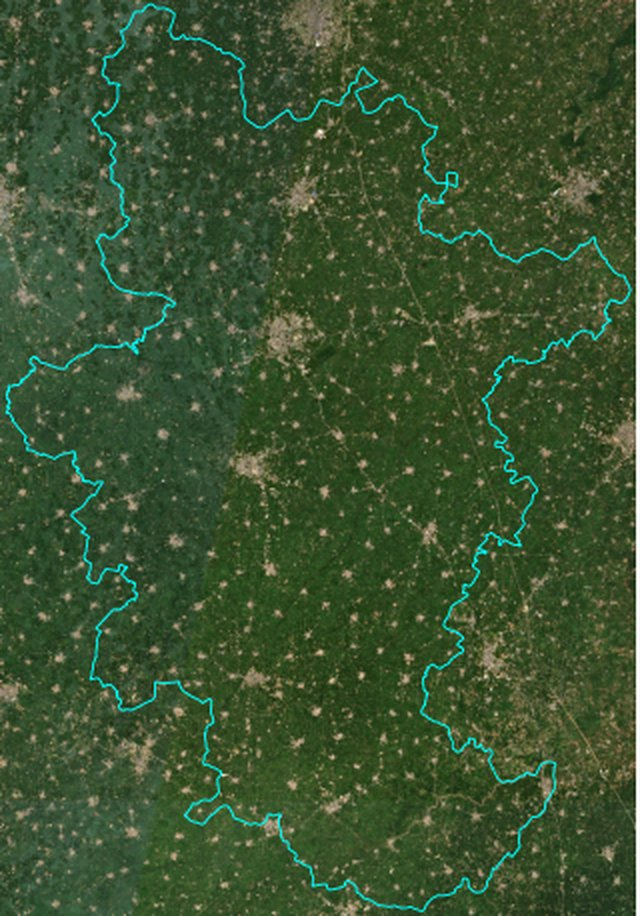
\includegraphics[width=0.78\columnwidth]{study_area.jpg}
\caption{Sangrur district (cyan outline), Sentinel-2 true-colour pre-season median composite,
20~Sep--5~Oct 2025.}
\label{fig:study}
\end{figure}

\begin{figure}[t]
\centering
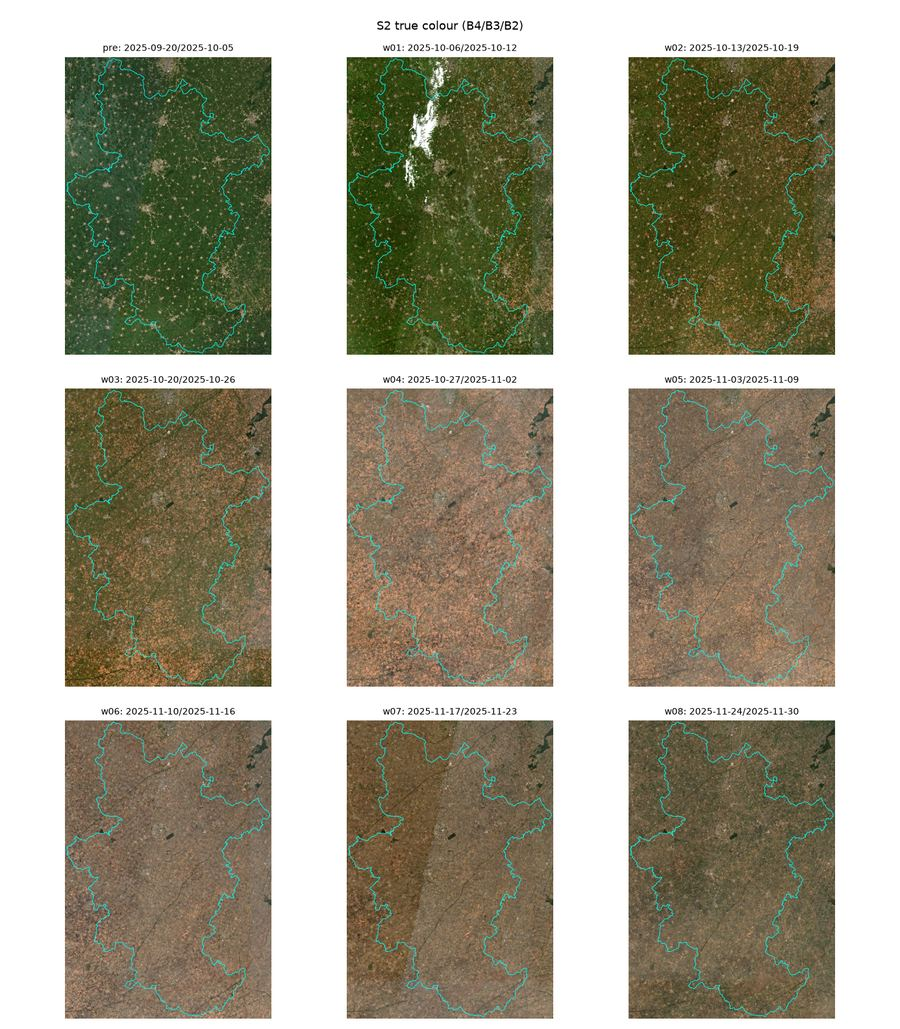
\includegraphics[width=0.92\columnwidth]{weekly_composites.jpg}
\caption{Sentinel-2 true-colour median composites (M1) for the pre-season window and weeks
w01--w08 (cyan: district boundary). Green paddy turns into harvested and burnt fields from w03;
w01 contains cloud.}
\label{fig:composites}
\end{figure}

\textbf{Season and weeks.} The season is 1~October--30~November 2025. A pre-season window
(20~Sep--5~Oct) gives the reference state. Reporting weeks are w00 = 1--5~Oct and then w01--w08,
7-day windows from 6~October (w08 = 24--30~Nov).

\textbf{Sentinel-2.} Level-2A surface reflectance from the Microsoft Planetary
Computer~\cite{mpc}, bands B02, B03, B04, B08, B8A, B11 and B12, with the Sen2Cor scene
classification (SCL) and aerosol optical thickness (AOT)~\cite{mainknorn2017}. 37 acquisitions
between 20~September and 29~November were used. SCL classes 0, 1, 3, 8, 9 and 10 are treated as
invalid; class 2 (dark area) is deliberately kept because fresh burn scars are often put in it.

\textbf{Sentinel-1.} Radiometrically terrain-corrected VV and VH backscatter~\cite{torres2012}
(6 acquisitions in the pre-season window, 2--3 per week afterwards). Sentinel-1 is stored per
polygon as supporting evidence only; it never creates or removes a candidate.

\textbf{Ancillary.} ESA WorldCover 10~m~\cite{zanaga2022} for selecting pseudo-invariant pixels.

\textbf{FIRMS.} VIIRS 375~m active-fire detections from S-NPP and NOAA-20, standard-processing
archive (\texttt{VIIRS\_SNPP\_SP}, \texttt{VIIRS\_NOAA20\_SP}), fetched through the FIRMS area API
in 5-day requests for the district bounding box and clipped to the boundary: 857 detections
(S-NPP 420, NOAA-20 437). Detections from the two satellites are not merged, so one fire can
appear twice. Times are converted to IST (UTC+5:30).

% =========================================================================================
\section{Methodology}
Fig.~\ref{fig:pipeline} summarises the pipeline. Every intermediate file has a provenance sidecar
recording the code version and parameters, and cached downloads are never repeated.

\begin{figure}[t]
\centering
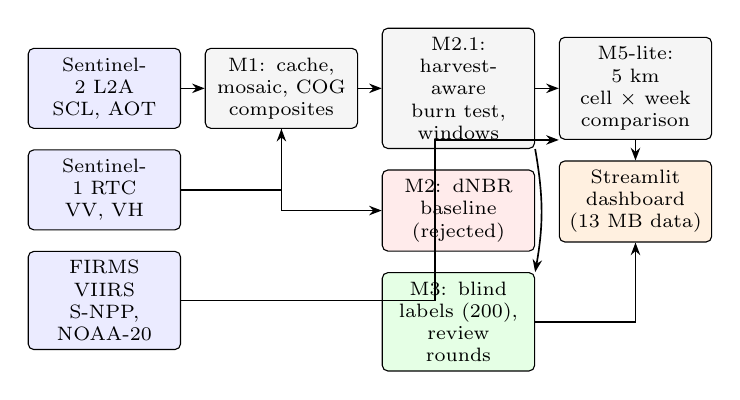
\begin{tikzpicture}[
  node distance=2.6mm and 3mm,
  box/.style={draw, rounded corners=2pt, align=center, font=\scriptsize,
              minimum height=7mm, text width=17mm, fill=#1},
  box/.default={gray!8},
  arr/.style={-{Stealth[length=1.6mm]}, semithick}]
\node[box=blue!8] (s2) {Sentinel-2 L2A\\SCL, AOT};
\node[box=blue!8, below=of s2] (s1) {Sentinel-1 RTC\\VV, VH};
\node[box=blue!8, below=of s1] (fi) {FIRMS VIIRS\\S-NPP, NOAA-20};
\node[box, right=of s2] (m1) {M1: cache,\\mosaic, COG\\composites};
\node[box, right=of m1] (m21) {M2.1: harvest-\\aware burn test,\\windows};
\node[box=red!8, below=of m21] (m2) {M2: dNBR\\baseline\\(rejected)};
\node[box=green!10, below=of m2] (m3) {M3: blind\\labels (200),\\review rounds};
\node[box, right=of m21] (m5) {M5-lite: 5~km\\cell $\times$ week\\comparison};
\node[box=orange!12, below=of m5] (dash) {Streamlit\\dashboard\\(13~MB data)};
\draw[arr] (s2) -- (m1); \draw[arr] (s1) -| (m1);
\draw[arr] (m1) -- (m21); \draw[arr] (m1) |- (m2);
\draw[arr] (m21) -- (m5); \draw[arr] (m21.south east) to[bend left=10] (m3.north east);
\draw[arr] (fi) -- ++(4.2,0) |- (m5.south west);
\draw[arr] (m5) -- (dash); \draw[arr] (m3) -| (dash);
\end{tikzpicture}
\caption{Processing pipeline. Sentinel-1 is attached to polygons as supporting evidence only.}
\label{fig:pipeline}
\end{figure}

\subsection{M1: Data pipeline and compositing}
The catalogue is searched for every Sentinel-2 and Sentinel-1 item intersecting the district in
the season. Each acquisition is mosaicked onto the 10~m district grid and cached as a GeoTIFF. Two
Sentinel-2 passes on the same day are merged by the mean of their clear observations. For quick
looks and the baseline, per-window median composites are written as Cloud-Optimised GeoTIFFs with an
observation-count band (Fig.~\ref{fig:composites}). These counts exposed the observation gaps early: in w04
(27~Oct--2~Nov) only 27.5\,\% of the district had two or more clear Sentinel-2 views, against
99.8\,\% in w05. Detection itself does not use weekly composites; it scans each pixel's full time
series of clear views.

\subsection{M2: dNBR baseline and why it measured harvest}
The project brief specified a baseline of
$\mathrm{NBR}=(B8-B12)/(B8+B12)$~\cite{keybenson2006} and
$\mathrm{dNBR}=\mathrm{NBR}_{\mathrm{pre}}-\mathrm{NBR}_{\mathrm{obs}}$ with
$\mathrm{NBR}_{\mathrm{pre}}$ the per-pixel pre-season median. A pixel was a candidate on its first
clear day with $\mathrm{dNBR}>0.27$. After a $3\times3$ opening and removal of patches under
0.1~ha, the baseline flagged \textbf{236{,}566~ha, 80.6\,\% of the district}, in 236{,}415
polygons (Fig.~\ref{fig:m2}). The scene-wide median NBR of clear pixels falls from about 0.6 in the
pre-season window (standing paddy) to about $-0.1$ by November. A drop of that size exceeds 0.27
for every harvested field, burnt or not, so the first-detection date tracks harvest. 59{,}776~ha
of candidates showed only a gradual NBR decline between consecutive clear looks, which fits
harvest or senescence better than an abrupt burn. The baseline was therefore kept only as a
reference and not reported as burnt area.

\begin{figure}[t]
\centering
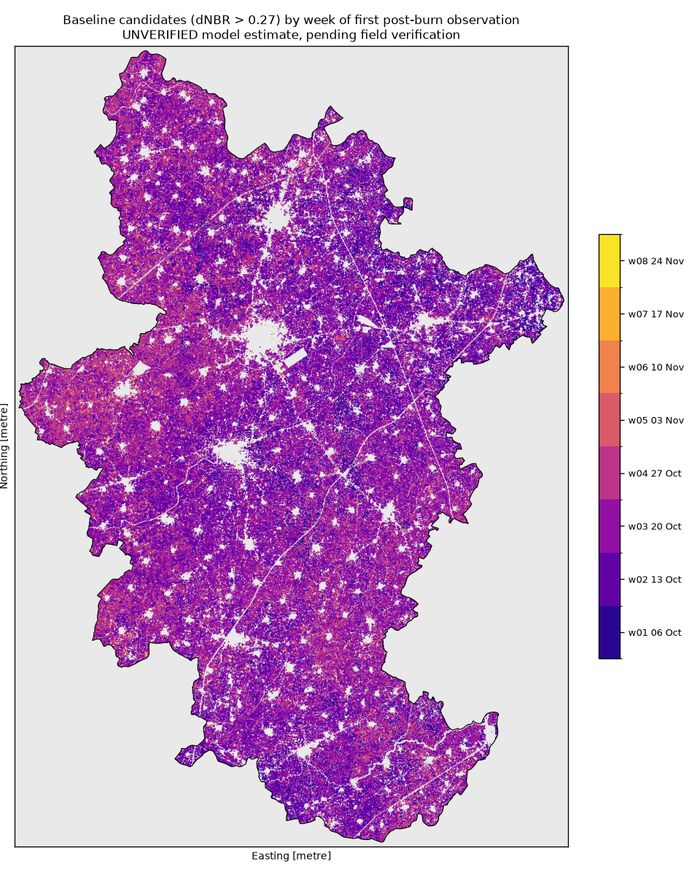
\includegraphics[width=0.72\columnwidth]{m2_baseline.jpg}
\caption{M2 baseline candidates (pre-season dNBR $>0.27$) by week of first detection. The
baseline flags 80.6\,\% of the district and largely tracks harvest.}
\label{fig:m2}
\end{figure}

\subsection{M2.1: Harvest-aware detection}
M2.1 first finds each pixel's harvest: the first usable clear view with $\mathrm{NDVI}<0.3$ after at
least one view with $\mathrm{NDVI}>0.6$. A burn is then tested only between \emph{consecutive}
usable views after that harvest view, so the harvest drop itself can no longer trigger a
detection. All three conditions must hold between the two views: NBR drop $>0.10$, relative albedo
drop $>0.15$ (albedo = mean of B02, B03, B04, B08), and NBR2 drop $>0.02$, with
$\mathrm{NBR2}=(B11-B12)/(B11+B12)$. Thresholds were fixed in configuration before the run and not
tuned to the result.

\textbf{Haze and smoke.} A clear-by-SCL view is skipped as hazy if B02 $>0.15$, if it lies within
300~m of SCL cloud, or if Sen2Cor AOT $>0.6$. Skipped views widen burn-date windows but never
trigger a burn. A scene rule fixed before the run drops a whole date if fewer than 20\,\% of its
SCL-clear pixels survive the haze mask or its residual spread on pseudo-invariant pixels exceeds
three times the median. This dropped 30~October and 22~November. The 28~October scene was only
1.4\,\% SCL-clear over the district.

\textbf{Radiometric normalisation.} For each acquisition and band, the median deviation of
84{,}724 pseudo-invariant pixels (WorldCover built-up and bare classes, eroded, NDVI max
$<0.3$, low relative spread) from their season median is subtracted before any index is computed.

\textbf{Early burns.} If the first non-green view is already very dark
($\mathrm{NBR}\le-0.24$ and albedo $\le0.09$, the 25th percentile of earlier M2.1 burns), the pixel
is labelled \texttt{harvest\_and\_burn\_same\_window} (672 polygons, 288~ha). Pixels with a harvest
view but no usable view afterwards are \texttt{unobserved} (283~ha) and are never reported as not
burnt. Cleaning is as in M2, and polygons are split by date of first burnt view, so one polygon is
one detection event.

\subsection{Burn-date windows}
Each candidate carries a burn-date window [last clear unburnt view, first clear burnt view],
inclusive at both ends because a fire after the 10:30~IST Sentinel-2 overpass is possible. The end
of the window, \texttt{detect\_date}, is the first view showing the scar, not the burn date. All
weekly reporting uses the week of \texttt{detect\_date}. (An earlier stored attribute,
\texttt{week\_detected}, placed 912 polygons, about 420~ha, first seen before 6~October into w08;
it is not used anywhere in the results or the dashboard.) Windows are wide where views are
missing: 80{,}637~ha of candidates have a window overlapping w04, but only 166~ha have the whole
window inside it (Fig.~\ref{fig:w04}).

\begin{figure}[t]
\centering
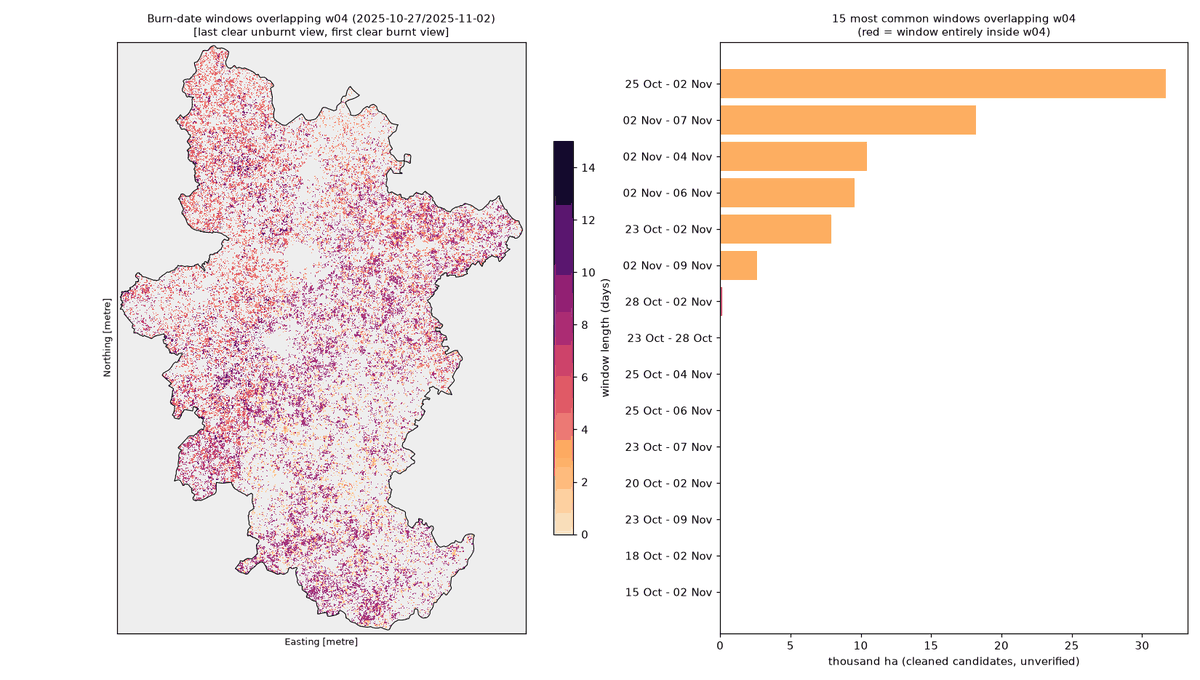
\includegraphics[width=\columnwidth]{w04_windows.png}
\caption{Burn-date windows of candidates overlapping w04 (27~Oct--2~Nov). Missing and hazy
late-October views stretch most windows across the week boundary.}
\label{fig:w04}
\end{figure}

\subsection{Quality bands}
Per pixel and per polygon the pipeline stores the number of clear Sentinel-2 days (season,
pre-season, post-detection and per week), days since the previous clear day, the longest gap, the
haze fraction at detection, the window width, supporting observations within 10~days after
detection, and the Sentinel-1 VV/VH change. Flags include \texttt{single\_observation} (1{,}138
polygons, 456~ha in M2.1), \texttt{haze\_at\_detection} and wide windows ($>10$~days). A
rule-based \texttt{detection\_score}, the polygon mean of the smallest of the three drop-to-threshold
ratios, ranks candidates; it is not a probability, and \texttt{burn\_confidence} is left empty until a
calibrated model exists.

\textbf{Outcome.} M2.1 flagged \textbf{135{,}979~ha (46.3\,\% of the district, 54.5\,\% of the
249{,}606~ha harvested)} in 97{,}137 polygons (Table~\ref{tab:oldnew}, Fig.~\ref{fig:m21}). A
sensitivity test on six sample blocks shows the dependence on thresholds: halving or doubling the
NBR-drop threshold moves the burnt share of harvested pixels from 61.1\,\% to 65.7\,\% or 42.0\,\%,
and shifting the harvest NDVI threshold by $\pm0.05$ moves it to 49.8\,\% or 65.8\,\%. Without
labels the thresholds cannot be tuned.

\begin{table}[t]
\caption{Baseline vs harvest-aware detection (district totals)}
\label{tab:oldnew}
\centering
ootnotesize
\begin{tabular}{@{}lrrr@{}}
\toprule
Method & Area (ha) & \% AOI & Polygons \\
\midrule
M2 baseline, dNBR $>0.27$ & 236{,}566 & 80.6 & 236{,}415 \\
M2.1 frozen (blue haze only) & 138{,}678 & 47.2 & 101{,}894 \\
M2.1 + AOT, PIF, early burns & 135{,}979 & 46.3 & 97{,}137 \\
\bottomrule
\end{tabular}
\end{table}

\begin{figure}[t]
\centering
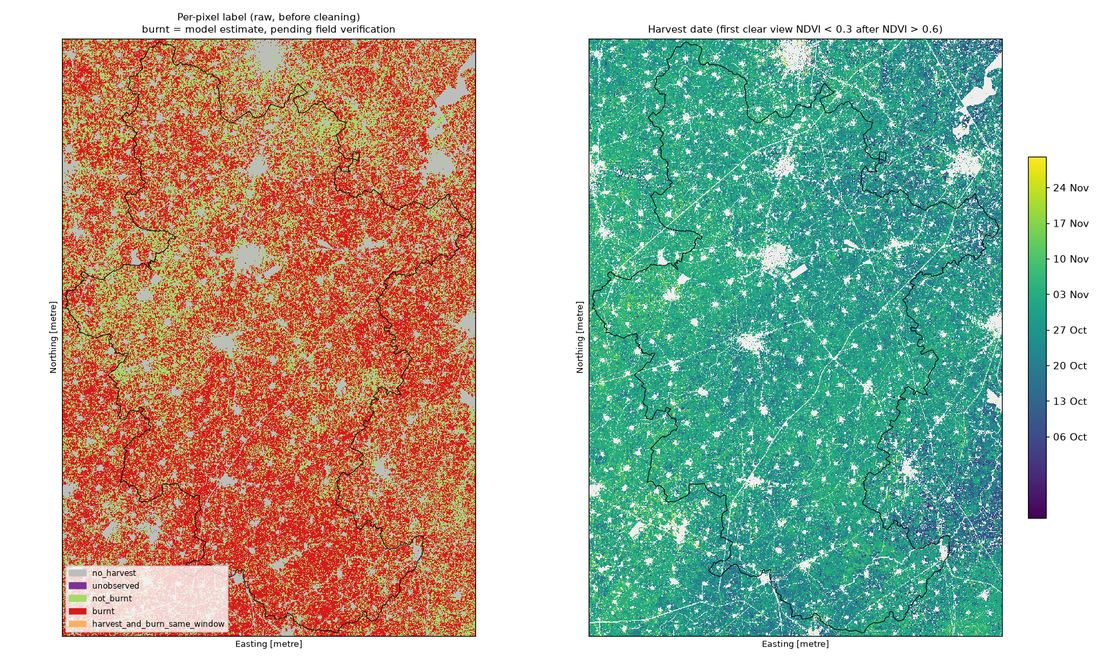
\includegraphics[width=\columnwidth]{m21_labels.jpg}
\caption{M2.1 per-pixel label before cleaning (left; burnt = model estimate, pending field
verification) and harvest date (right).}
\label{fig:m21}
\end{figure}

% =========================================================================================
\section{Validation Study}
\subsection{Sample design}
A seeded, stratified random sample of 400 items was drawn before labelling: 320 M2.1 polygons
stratified by five detection-score bins and eight weeks (w04 double-weighted because of its
observation gaps), and 80 unflagged cropland cells of 1~ha in nine week strata. Items were labelled
in a fixed random order; the first \textbf{200} were labelled (159 candidates, 41 unflagged cells).
Each item keeps a subset inclusion weight (stratum population over items labelled from it) for
design-weighted estimates. The labeller saw no model output, score or stratum.

\subsection{Labelling tool}
A purpose-built Streamlit tool shows, for a crosshair inside the item, a time strip of every clear
Sentinel-2 view as true colour, SWIR false colour and $\Delta$NBR from the previous date, with a chart
of NBR, albedo and NDVI at the crosshair (Fig.~\ref{fig:tool}). Labels are \texttt{burnt},
\texttt{not\_burnt} or \texttt{unsure}, with an optional burn date (first date the field turns
dark), stored append-only in SQLite. Twenty items were repeated at least 40 positions later as
hidden repeats shown \emph{without} the chart and $\Delta$NBR row (imagery only), which gives both a
self-agreement and a chart-on/off test. Chart-on (first-showing) labels are the primary labels.

\begin{figure}[t]
\centering
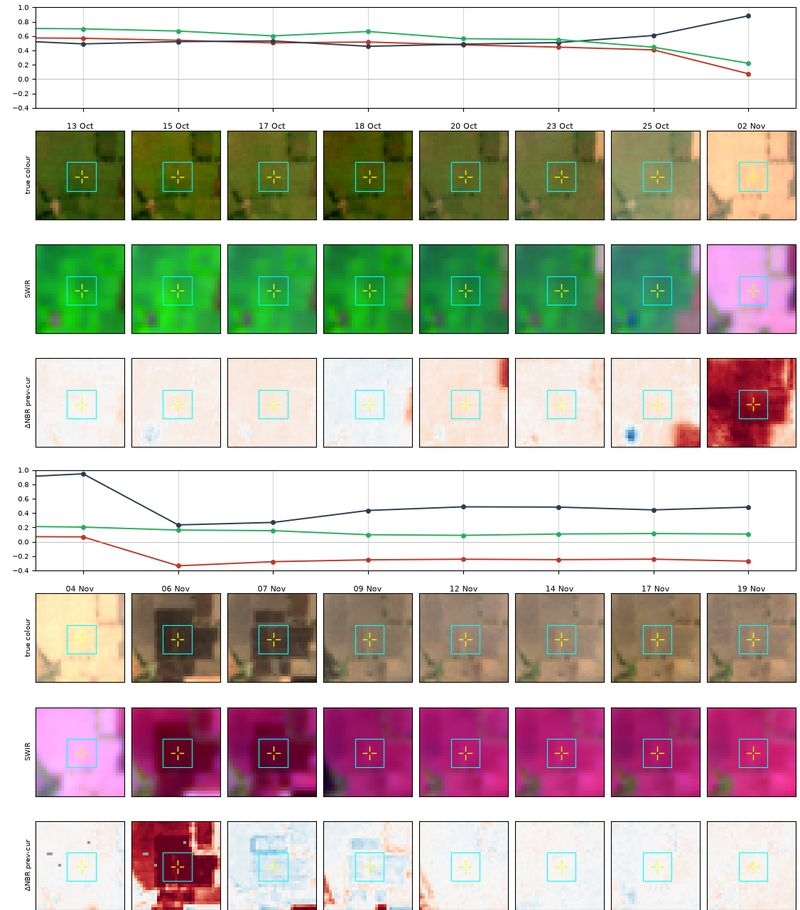
\includegraphics[width=0.92\columnwidth]{label_tool.jpg}
\caption{Part of a labelling-tool strip: chart of NBR (red), albedo$\times$4 (dark) and NDVI
(green) at the crosshair, and true colour, SWIR and $\Delta$NBR chips per clear date. The field
darkens between 2 and 6~November.}
\label{fig:tool}
\end{figure}

\subsection{Review rounds}
A timing check showed many labels saved within 2~s of the previous one. In review round r1 the 97
fast items and 20 slow control items were shown again blind, in random order, with a 4~s delay
before saving. 57 of 96 reviewed fast items changed (59\,\%, 95\,\% Wilson CI~\cite{wilson1927}
49--69\,\%) and 10 of 20 controls changed (50\,\%, CI 30--70\,\%), mostly \texttt{not\_burnt}
$\rightarrow$ \texttt{burnt} (52 and 8). Because the controls changed as often as the fast items,
speed was not the only problem, and round r2 re-showed the remaining 103 unreviewed items blind,
now requiring a burn date for every \texttt{burnt} label, plus a date-only pass over 35 earlier
burnt items. In r2, 71 of 103 changed (69\,\%, CI 59--77\,\%; 54 \texttt{not\_burnt}
$\rightarrow$ \texttt{burnt}) and 5 of 35 in the date pass. Final labels: 134 burnt, 57 not burnt,
9 unsure; all 143 current burnt labels have a burn date.

\subsection{Agreement and the chart effect}
On the 20 hidden repeat pairs the labeller agreed with themself 55\,\% of the time, Cohen's
$\kappa=0.17$~\cite{cohen1960} (burnt vs not burnt only: 57.9\,\%, $\kappa=0.17$, 19 pairs). Of 7
pairs where both showings had a date, 4 had the same date. With the chart the burnt rate was
65\,\%, without it 45\,\%. Among 19 discordant-eligible pairs, 6 were burnt only with the chart and
2 only without; the exact McNemar test~\cite{mcnemar1947} gives $p=0.289$, so the sample is too
small to show a chart effect, but the direction is consistent with the chart pulling labels towards
the rule (labels matched the M2.1 flag in 68.4\,\% of pairs with the chart vs 60\,\% without).

\subsection{Results against M2.1}
Unweighted, 112 of 159 candidates were labelled burnt (70.4\,\%, CI 62.9--77.0\,\%) and 22 of 41
unflagged cells (53.7\,\%, CI 38.7--67.9\,\%). Design-weighted to the sampling frame, M2.1 polygons
were burnt in 76\,\% of cases by count and 90\,\% by area; unflagged cropland cells were burnt in
38\,\%, which suggests M2.1 also misses burns. Of the 112 candidates labelled burnt, the labelled
burn date falls inside the detected window for 61 and the windows overlap for 76.
Because self-agreement is low and labels moved strongly towards \texttt{burnt} across the review
rounds, these shares are indicative only and are not used to correct the area.

% =========================================================================================
\section{Results}
\subsection{Burnt area}
Of the 135{,}979~ha flagged, 331 polygons (133~ha) were first seen before 1~October, leaving
\textbf{135{,}835~ha} of \AREA{} in the season. The weekly distribution (Table~\ref{tab:weekly})
peaks in w05 (3--9~Nov, 69{,}473~ha) after w04 (39{,}829~ha).

\begin{table}[t]
\caption{Weekly \AREA{} and VIIRS detections, by week of \texttt{detect\_date} and IST date}
\label{tab:weekly}
\centering
\small
\begin{tabular}{@{}llrr@{}}
\toprule
Week & Dates (2025) & Area (ha) & Hotspots \\
\midrule
w00 & 1--5 Oct & 287 & 5 \\
w01 & 6--12 Oct & 321 & 2 \\
w02 & 13--19 Oct & 2{,}132 & 9 \\
w03 & 20--26 Oct & 4{,}646 & 80 \\
w04 & 27 Oct--2 Nov & 39{,}829 & 416 \\
w05 & 3--9 Nov & 69{,}473 & 280 \\
w06 & 10--16 Nov & 15{,}076 & 61 \\
w07 & 17--23 Nov & 3{,}537 & 4 \\
w08 & 24--30 Nov & 535 & 0 \\
\midrule
Season & & 135{,}835 & 857 \\
\bottomrule
\end{tabular}
\end{table}

\subsection{Comparison with FIRMS}
Hotspots peak one week before the area estimate (w04 vs w05, Fig.~\ref{fig:weekly}). This fits the
Sentinel-2 gaps: with 28~October nearly fully cloudy and 30~October excluded, burns of late October
are first seen on 2~November or later. Per 5~km cell, the Spearman rank correlation between
estimated area and hotspot count is 0.55: both concentrate in the centre and south of the district
(Fig.~\ref{fig:grid}, Fig.~\ref{fig:scatter}). The season has about 159~ha of estimated area per
detection, but a VIIRS detection is a 375~m pixel seen at two moments a day, not an area, so this
ratio is not an undercount factor. Cells whose share of hotspots is far below their share of area
(e.g.\ SGR-G-127, -124, -117, -043, -107: 1{,}284--1{,}486~ha each with 1--2 detections) are
prompts for field checks. A mismatch can come from off-pass burning, false positives (tilled or
wet soil), fires too small or short for VIIRS, or cloud and haze; it is not a finding about any
village.

\begin{figure}[t]
\centering
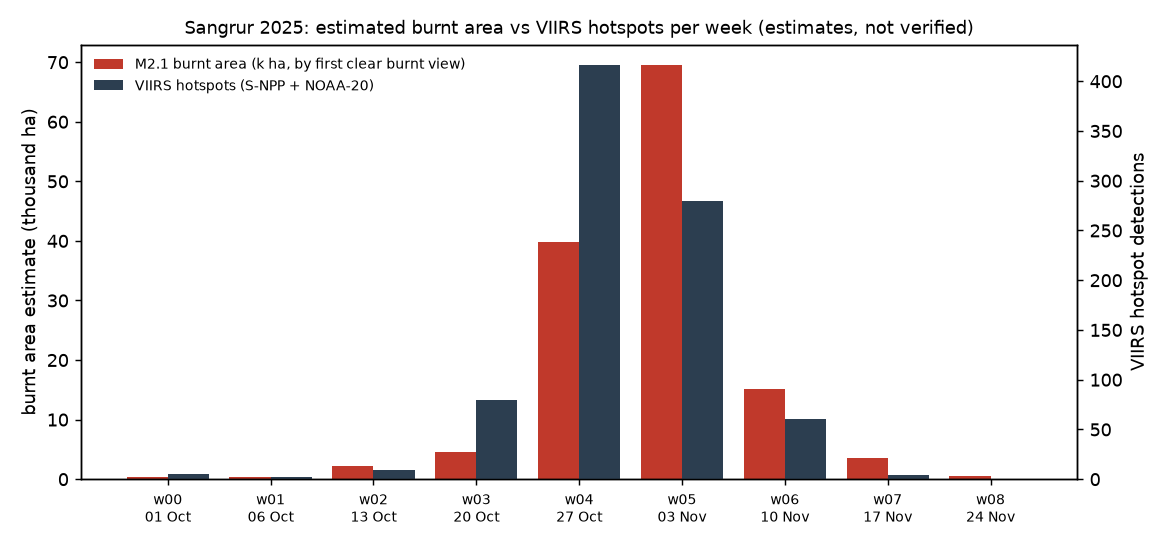
\includegraphics[width=\columnwidth]{weekly.png}
\caption{Weekly \AREA{} (bars) and VIIRS S-NPP + NOAA-20 detections (line).}
\label{fig:weekly}
\end{figure}

\begin{figure*}[t]
\centering
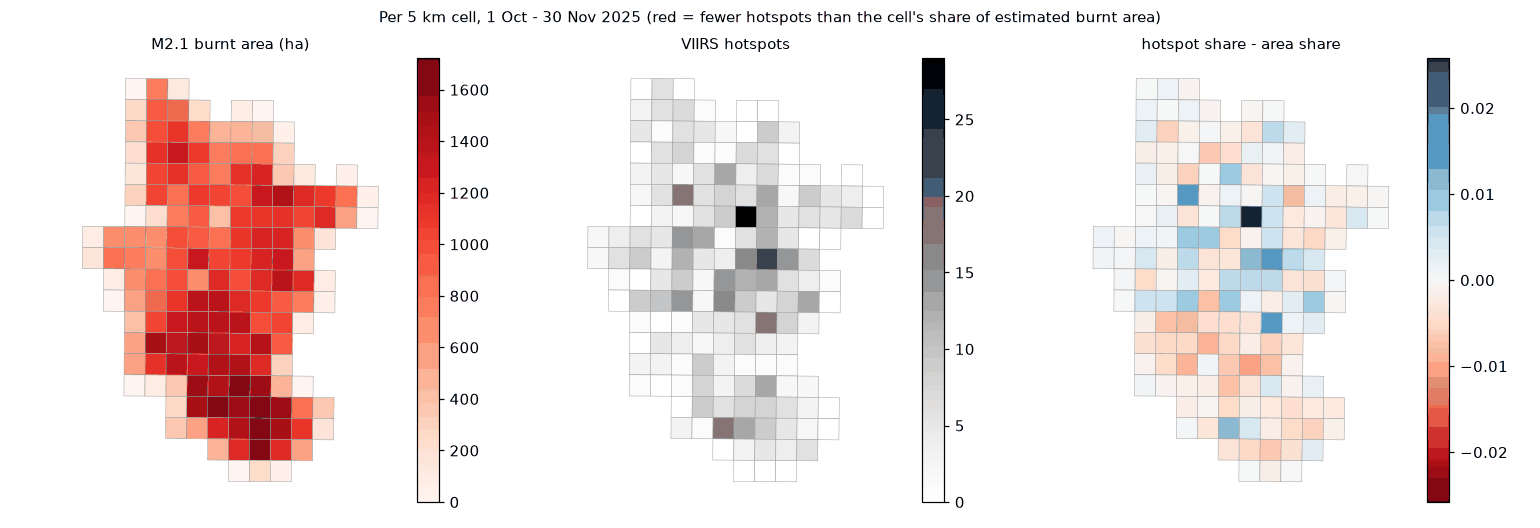
\includegraphics[width=0.9\textwidth]{grid_maps.png}
\caption{Per 5~km cell, 1~Oct--30~Nov 2025: \AREA{} (left), VIIRS detections (centre) and hotspot
share minus area share (right; red = fewer hotspots than the cell's share of estimated area).}
\label{fig:grid}
\end{figure*}

\begin{figure}[t]
\centering
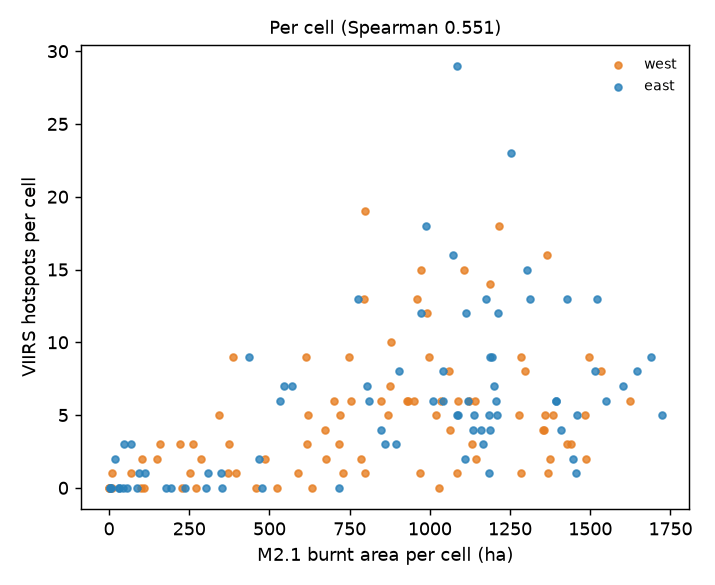
\includegraphics[width=0.85\columnwidth]{scatter.png}
\caption{Per cell: \AREA{} vs VIIRS detections (Spearman $\rho=0.55$, 162 cells).}
\label{fig:scatter}
\end{figure}

\subsection{Hour of detection}
852 of the 857 detections were made between 12:00 and 14:59~IST (12~h: 94, 13~h: 528, 14~h: 230)
and the other 5 between 01:00 and 02:59~IST (Fig.~\ref{fig:hours}). VIIRS thus samples two short
windows of the day. Singh \emph{et al.}~\cite{singh2025} report that peak burning shifted from
about 13:30 to about 17:00~IST between 2020 and 2024; a fire lit and extinguished in the late
afternoon falls between these passes. Our data alone cannot show how much burning happens off-pass,
but the burn scar remains visible to Sentinel-2 in either case.

\begin{figure}[t]
\centering
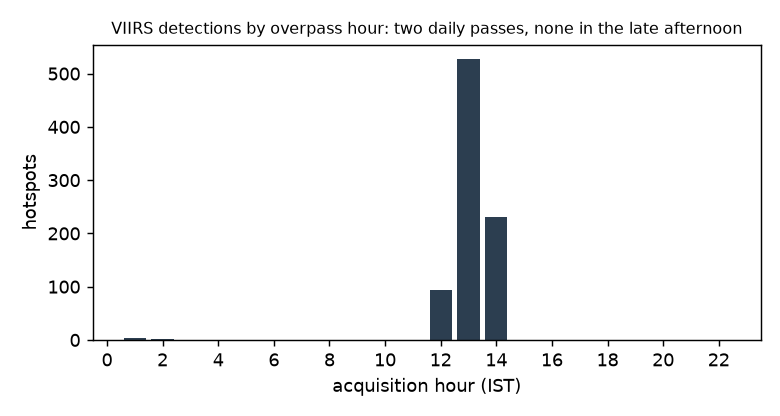
\includegraphics[width=0.95\columnwidth]{hours.png}
\caption{VIIRS detections in the district by IST hour. Peak burning has been reported to have
shifted from 13:30 to 17:00~IST between 2020 and 2024 (ISRO SAC, Current Science~\cite{singh2025}).}
\label{fig:hours}
\end{figure}

\subsection{West vs east}
Splitting the grid at the easting of the bounding-box midpoint, the west has 69{,}321~ha of estimated area,
414 detections and 85 cells; the east 66{,}514~ha, 443 detections and 77 cells. M2.1 polygons in the
west average 21.2 clear Sentinel-2 views against 30.1 in the east (median over cells 29.8). Fewer
views mean wider burn-date windows and a higher chance of missing short-lived scars, so west-side
estimates are less certain.

% =========================================================================================
\section{Deployment}
The results are published as a Streamlit dashboard on Streamlit Community Cloud
(\liveurl; code at \repourl). The heavy pipeline (geospatial stack, rasters of several GB) runs
offline; the command \texttt{stubble deploy-data} writes a small package of precomputed files
(13~MB, limit 50~MB) to \texttt{deploy/data/}, which is committed to the repository. The app reads
only that folder and depends on five pinned packages (Streamlit, pandas, NumPy, Altair, pydeck; no
deep-learning or GDAL stack), which keeps the free-tier build small.

The package holds the 5~km grid with per-week area and hotspot columns, the 857 FIRMS points, all
96{,}806 in-season candidates as centroids, the 4{,}427 largest polygons ($\ge5.3$~ha, 52{,}181~ha,
simplified to 10~m) fitted to an 8~MB browser budget, and the 200 labelled items as crosshair points
without field geometry. The Map page (Fig.~\ref{fig:dash}) has a week slider and layers for
polygons coloured by week, all candidates, hotspots and the labelled sample. The Weekly page shows
the area-vs-hotspot chart, the IST-hour chart with its citation, the grid maps and the west/east
table. The Method \& limitations page carries the full disclaimer, the validation numbers and the
ethics statement. Weeks always come from \texttt{detect\_date}, and every chart and map labels the
area as ``\AREA''.

\begin{figure}[t]
\centering
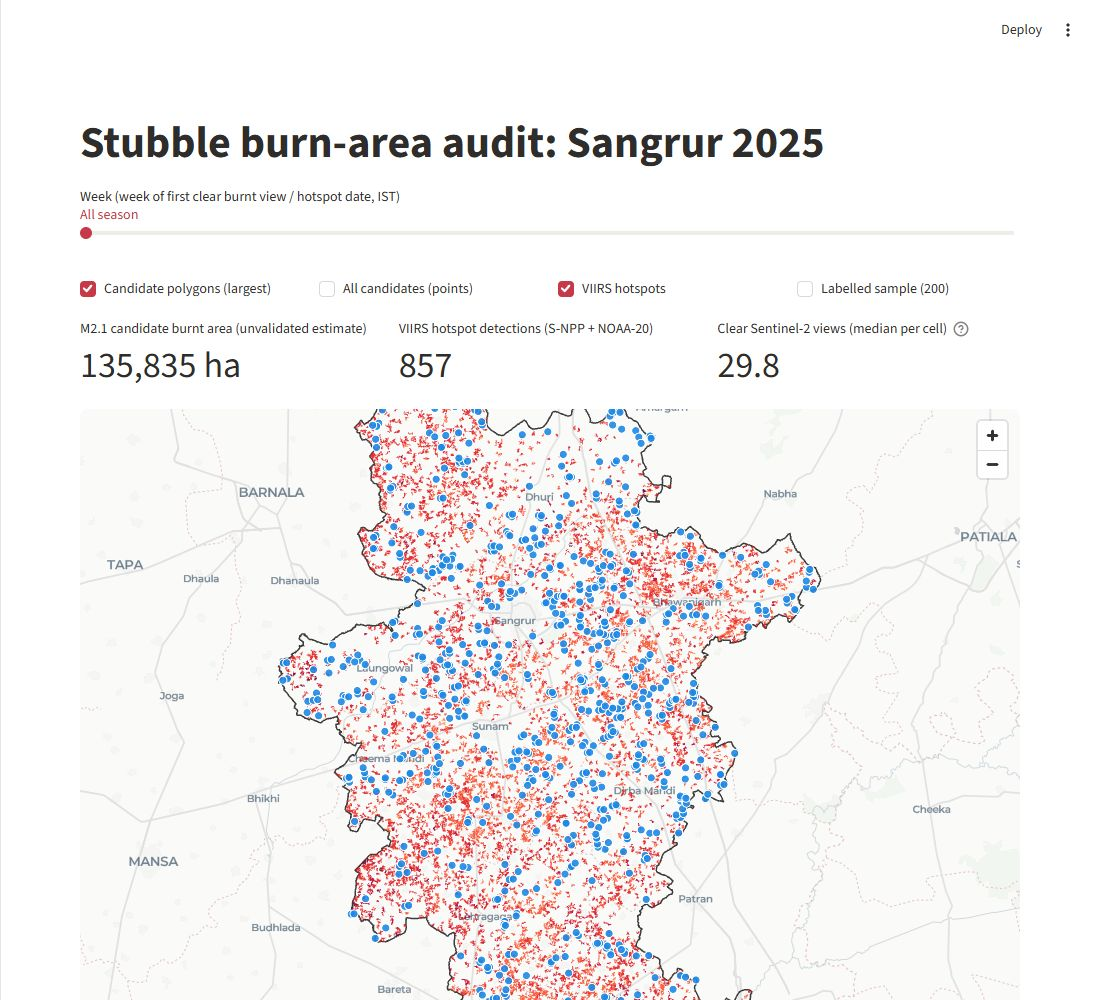
\includegraphics[width=\columnwidth]{dash_map.jpg}
\caption{Dashboard Map page: \AREA{} polygons (red) and VIIRS detections (blue), season view.}
\label{fig:dash}
\end{figure}

% =========================================================================================
\section{Limitations and Ethics}
\subsection{Limitations}
\begin{itemize}
\item \textbf{Label reliability.} One labeller, no field visits; self-agreement 55\,\%
($\kappa=0.17$) on 20 pairs, and large shifts towards \texttt{burnt} across review rounds. No
precision or recall is claimed. The labelling chart shows the same indices the rule uses and may
pull labels towards it (McNemar $p=0.289$, not significant at $n=20$).
\item \textbf{Resolution.} At 10--20~m, small fields and mixed pixels at bunds are not resolved;
adjacent fields with the same detection date merge into one polygon.
\item \textbf{Haze and smoke.} The 28~October scene was 1.4\,\% clear and 30~October was excluded,
which shifts first detections into November and widens windows. Sen2Cor AOT is nearly constant
within a scene (median p10--p90 width 0.04), so it flags hazy scenes, not local smoke plumes.
\item \textbf{Tilled vs burnt.} Tillage that incorporates straw, or wet soil, can lower NBR,
albedo and NBR2 together, like a burn. The three-way test reduces but does not remove this.
\item \textbf{Observation gaps in the west.} About 21 clear views per candidate in the west vs 30
in the east; western windows are wider and short-lived scars more easily missed.
\item \textbf{Hotspots are not area.} S-NPP and NOAA-20 duplicates are not merged; MODIS and
NOAA-21 are not included.
\item \textbf{Threshold dependence.} Area shifts by tens of percent under plausible threshold
changes, and thresholds could not be tuned without reliable labels.
\end{itemize}

\subsection{Ethics}
The system is decision support only. It contacts no one, triggers no fines and supports no
automated enforcement; every polygon has status \texttt{pending\_field\_verification} until a human
changes it, and the UI never presents an output as confirmed fact. No personal data is used: no
owner names, phone numbers or land records; fields have synthetic IDs derived from geometry (e.g.\
\texttt{SGR-0001}), and the public dashboard shows labelled items as points without field outlines.
Grid cells with mismatches are framed as prompts for verification, not as findings about
villages. Only open data is used, and API keys are kept out of the repository.

% =========================================================================================
\section{Conclusion and Future Work}
A conventional dNBR threshold over-flags paddy districts because harvest itself drops NBR
strongly. Testing for a burn only between consecutive clear views after each pixel's harvest, with
haze masking, radiometric normalisation and explicit burn-date windows, gives a plausible map
(135{,}835~ha in season) whose spatial pattern agrees moderately with VIIRS hotspots and whose
timing lags hotspots by the observation gap that late-October haze created. The validation study is
the weakest link: low labeller self-agreement means the area remains an unvalidated estimate.

Future work: (1)~\textbf{M4}: fine-tune a U-Net~\cite{ronneberger2015} initialised from
SSL4EO-S12 self-supervised Sentinel-2 weights~\cite{wang2023} on chips from the labels, with
spatially split train/validation/test tiles and calibrated per-polygon confidence; (2)~a label
re-test (r3) and a second labeller to measure inter-rater agreement before training; (3)~\textbf{photo
assessment after M4}: checking model outputs against photographs, to be designed once the model
exists; (4)~evidence packs per field for human verifiers; and (5)~merging
VIIRS duplicates and adding MODIS and NOAA-21.

% =========================================================================================
\begin{thebibliography}{99}
\bibitem{anand2025} A. Anand, R. Imasu, S. K. Dhaka, and P. K. Patra, ``Domain adaptation and
fine-tuning of a deep learning segmentation model of small agricultural burn area detection using
high-resolution Sentinel-2 observations: A case study of Punjab, India,'' \emph{Remote Sensing},
vol.~17, no.~6, Art.~no.~974, 2025, doi: 10.3390/rs17060974.

\bibitem{walker2022} K. Walker, B. Moscona, K. Jack, S. Jayachandran, N. Kala, R. Pande, J. Xue,
and M. Burke, ``Detecting crop burning in India using satellite data,'' arXiv:2209.10148, 2022.

\bibitem{singh2025} N. Singh, R. Pradhan, B. P. Shukla, and M. R. Pandya, ``Evidence of shift in
stubble burning timing over northwest India from geostationary satellite observations,''
\emph{Current Science}, vol.~129, no.~10, pp.~921--923, 2025,
doi: 10.18520/cs/v129/i10/921-923.

\bibitem{nrsc2023} Agro-ecosystem and Modeling Division, NRSC, ISRO, ``Assessment of paddy stubble
burnt area progression over Punjab \& Haryana, Kharif 2023,'' NRSC Science Story, Hyderabad,
India, 2023. [Online]. Available:
\url{https://www.nrsc.gov.in/nrscnew/assets/img/sciencestory/3_Science_Story_Stubble_burning_Pun_Har_2023.pdf}

\bibitem{trigg2001} S. Trigg and S. Flasse, ``An evaluation of different bi-spectral spaces for
discriminating burned shrub-savannah,'' \emph{Int. J. Remote Sens.}, vol.~22, no.~13,
pp.~2641--2647, 2001, doi: 10.1080/01431160110053185.

\bibitem{schroeder2014} W. Schroeder, P. Oliva, L. Giglio, and I. A. Csiszar, ``The new VIIRS
375\,m active fire detection data product: Algorithm description and initial assessment,''
\emph{Remote Sens. Environ.}, vol.~143, pp.~85--96, 2014, doi: 10.1016/j.rse.2013.12.008.

\bibitem{firms} NASA, ``Fire Information for Resource Management System (FIRMS).'' [Online].
Available: \url{https://firms.modaps.eosdis.nasa.gov}

\bibitem{drusch2012} M. Drusch \emph{et al.}, ``Sentinel-2: ESA's optical high-resolution mission
for GMES operational services,'' \emph{Remote Sens. Environ.}, vol.~120, pp.~25--36, 2012,
doi: 10.1016/j.rse.2011.11.026.

\bibitem{torres2012} R. Torres \emph{et al.}, ``GMES Sentinel-1 mission,'' \emph{Remote Sens.
Environ.}, vol.~120, pp.~9--24, 2012, doi: 10.1016/j.rse.2011.05.028.

\bibitem{mainknorn2017} M. Main-Knorn, B. Pflug, J. Louis, V. Debaecker, U. M\"uller-Wilm, and
F. Gascon, ``Sen2Cor for Sentinel-2,'' in \emph{Proc. SPIE 10427, Image and Signal Processing for
Remote Sensing XXIII}, 2017, doi: 10.1117/12.2278218.

\bibitem{mpc} Microsoft, ``Planetary Computer.'' [Online]. Available:
\url{https://planetarycomputer.microsoft.com}

\bibitem{zanaga2022} D. Zanaga \emph{et al.}, ``ESA WorldCover 10 m 2021 v200,'' Zenodo, 2022,
doi: 10.5281/zenodo.7254221.

\bibitem{keybenson2006} C. H. Key and N. C. Benson, ``Landscape assessment (LA): Sampling and
analysis methods,'' in \emph{FIREMON: Fire Effects Monitoring and Inventory System}, USDA Forest
Service, Gen. Tech. Rep. RMRS-GTR-164-CD, 2006, pp.~LA-1--LA-51.

\bibitem{wilson1927} E. B. Wilson, ``Probable inference, the law of succession, and statistical
inference,'' \emph{J. Amer. Statist. Assoc.}, vol.~22, no.~158, pp.~209--212, 1927,
doi: 10.1080/01621459.1927.10502953.

\bibitem{cohen1960} J. Cohen, ``A coefficient of agreement for nominal scales,'' \emph{Educ.
Psychol. Meas.}, vol.~20, no.~1, pp.~37--46, 1960, doi: 10.1177/001316446002000104.

\bibitem{mcnemar1947} Q. McNemar, ``Note on the sampling error of the difference between
correlated proportions or percentages,'' \emph{Psychometrika}, vol.~12, no.~2, pp.~153--157, 1947,
doi: 10.1007/BF02295996.

\bibitem{ronneberger2015} O. Ronneberger, P. Fischer, and T. Brox, ``U-Net: Convolutional networks
for biomedical image segmentation,'' in \emph{Proc. MICCAI}, LNCS vol.~9351, 2015, pp.~234--241,
doi: 10.1007/978-3-319-24574-4\_28.

\bibitem{wang2023} Y. Wang, N. A. A. Braham, Z. Xiong, C. Liu, C. M. Albrecht, and X. X. Zhu,
``SSL4EO-S12: A large-scale multi-modal, multi-temporal dataset for self-supervised learning in
Earth observation,'' arXiv:2211.07044, 2022.
\end{thebibliography}

\end{document}
